\chapter{YOLO}

YOLO, ovvero "You Only Look Once", è un diffuso algoritmo di rilevamento di oggetti in tempo reale.

YOLO unifica quello che un tempo era un processo a più fasi, utilizzando un'unica rete neurale per eseguire sia la classificazione sia la previsione dei riquadri di delimitazione (bounding box) degli oggetti rilevati.
Ogni bounding box è definita dalle coordinate che ne identificano posizione e dimensioni all'interno dell'immagine, oltre a un punteggio di confidenza e all'etichetta della classe dell'oggetto. In questo modo il modello è in grado di localizzare e classificare simultaneamente tutti gli oggetti presenti in una singola inferenza, formulando il problema come una regressione diretta delle coordinate dei bounding box e delle probabilità di appartenenza alle diverse classi.

È fortemente ottimizzato per le prestazioni di rilevamento e può operare molto più velocemente rispetto all'esecuzione di due reti neurali distinte per rilevare e classificare gli oggetti separatamente. Ciò avviene riadattando i classificatori di immagini tradizionali per la specifica attività di regressione volta a individuare i bounding box degli oggetti. \cite{yolo_info}

\newpage

\section{YOLO26}

YOLO26 è l'ultima famiglia unificata di modelli di visione in tempo reale.
Introduce l'inferenza nativa end-to-end, una head di rilevamento più leggera, una ricetta di addestramento aggiornata e head specifiche per compito per rilevamento, segmentazione, stima della posa, classificazione. \cite{yolo26_ultralytics}

\subsection{Versioni}

I modelli YOLO26, offrono diversi tagli per ogni versione del modello, passando dalla più piccola denominata "nano" (YOLO26n), alla più grande "extra large" (YOLO26x), nei quali differenza sta nella loro dimensione a livello di parametri.
Questa variazione di parametri ci permetti di aumentare le prestazioni, e quindi la qualità del modello.

\subsection{Metriche di valutazione}

Dopo aver addestrato un modello YOLO, dobbiamo misurarne le prestazioni ed eventualmente perfezionarlo per colmare le lacune.
La valutazione utilizza metriche come precision e la recall, le quali unite alla mAP ci permettono di quantificare l'accuratezza del modello. \\

\begin{table}[htbp]
    \centering
    \renewcommand{\arraystretch}{1.3}
    \begin{tabular}{lccccc}
        \toprule
        \textbf{Model} & 
        \textbf{\begin{tabular}[c]{@{}c@{}}mAP$_{50}$ \end{tabular}} &
        \textbf{\begin{tabular}[c]{@{}c@{}}mAP$_{95}$ \end{tabular}} &
        \textbf{\begin{tabular}[c]{@{}c@{}}Speed\\ \scriptsize{CPU}\\ \scriptsize{(ms)}\end{tabular}} & 
        \textbf{\begin{tabular}[c]{@{}c@{}}Speed\\ \scriptsize{GPU}\\ \scriptsize{(ms)}\end{tabular}} & 
        \textbf{\begin{tabular}[c]{@{}c@{}}params\\ \scriptsize{(M)}\end{tabular}} \\
        \midrule
        YOLO26n & 40.9 & 40.1 & $38.9 \pm 0.7$  & $1.7 \pm 0.0$  & 2.4  \\
        YOLO26s & 48.6 & 47.8 & $87.2 \pm 0.9$  & $2.5 \pm 0.0$  & 9.5  \\
        YOLO26m & 53.1 & 52.5 & $220.0 \pm 1.4$ & $4.7 \pm 0.1$  & 20.4 \\
        YOLO26l & 55.0 & 54.4 & $286.2 \pm 2.0$ & $6.2 \pm 0.2$  & 24.8 \\
        YOLO26x & 57.5 & 56.9 & $525.8 \pm 4.0$ & $11.8 \pm 0.2$ & 55.7 \\
        \bottomrule
    \end{tabular}
\end{table}
\cite{yolo26_ultralytics}

\newpage

\subsubsection{Precision}
La precision è la frazione di istanze rilevanti tra le istanze recuperate.

$$ Precision =\frac{\text{Istanze rilevanti recuperate}}{\text{Tutte le istanze recuperate}} = \frac{TP}{TP+FP} $$

\subsubsection{Recall}
La recall (anche nota come sensibilità) è la frazione di istanze rilevanti che sono state recuperate.

$$ Recall =\frac{\text{Istanze recuperate rilevanti}}{\text{Tutte le istanze rilevanti}} = \frac{TP}{TP+FN} $$

\noindent  \\ \\
Sia la precision che la recall si basano sull'output generato dal nostro modello. Queste metriche possono essere meglio rappresentate tramite questa immagine. 
\begin{figure}[htbp]
  \centering
  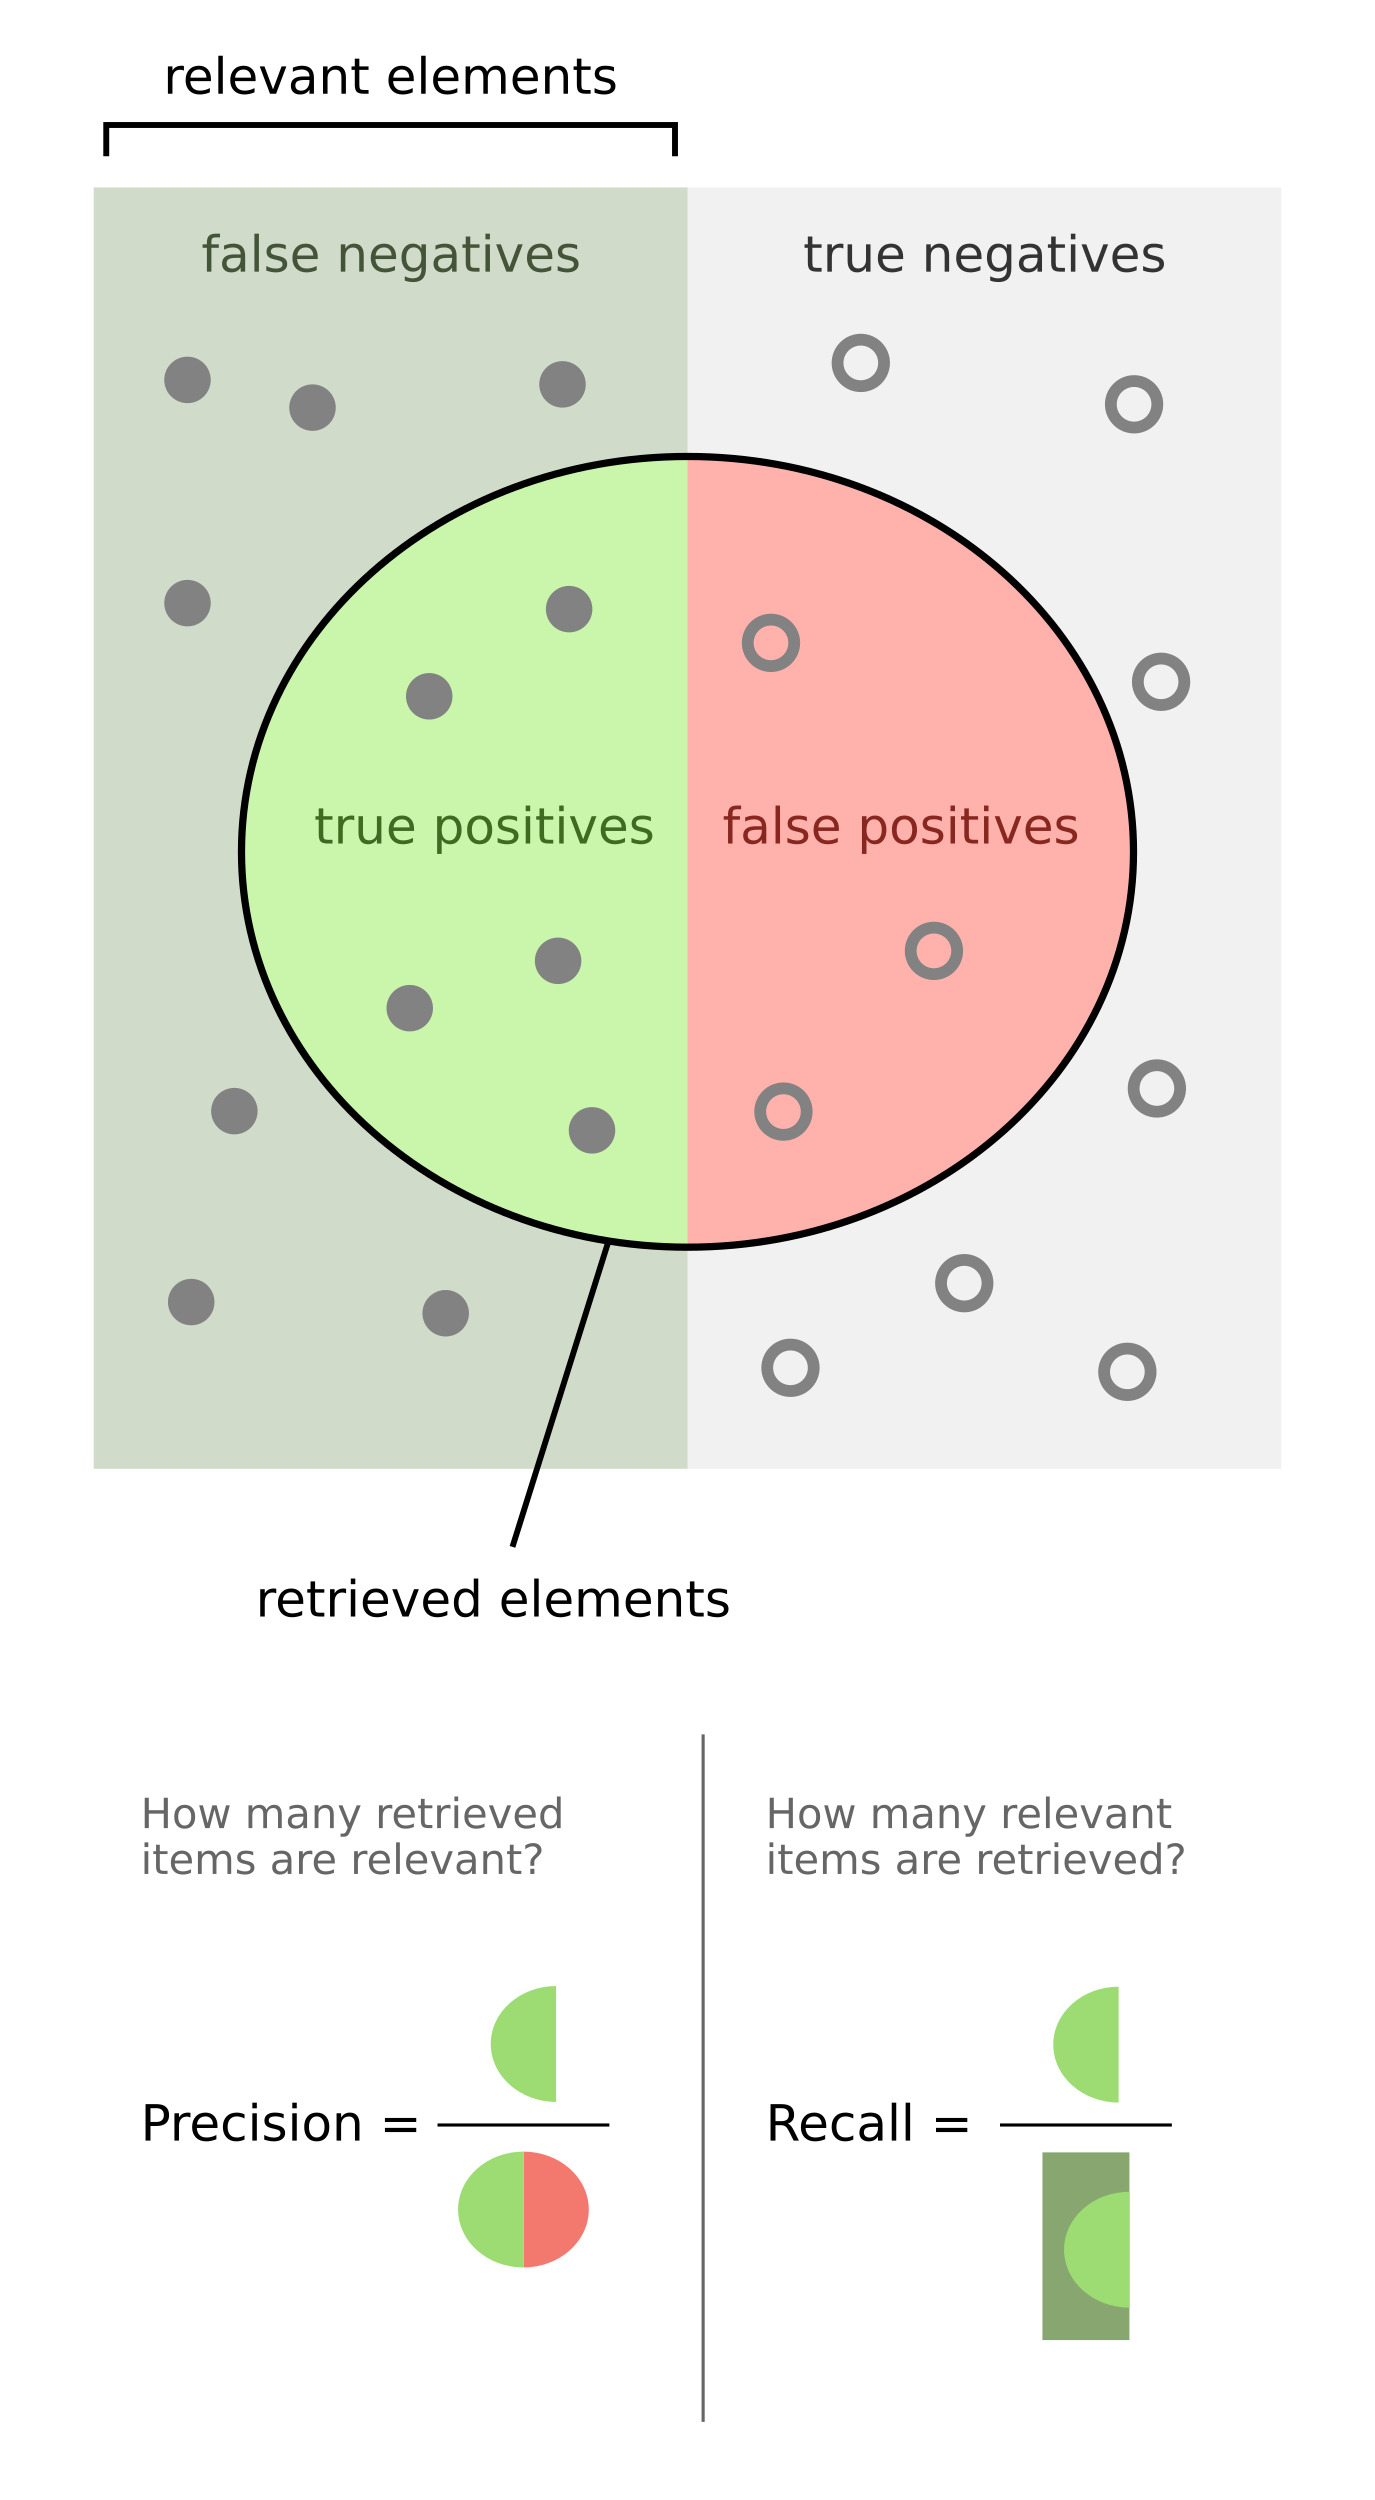
\includegraphics[width=0.8\textwidth]{images/precision-recall.jpg}
  \cite{precision_recall}
  \label{fig:precision_recall}
\end{figure}

\subsubsection{F1 score}
L'F1 score mette in rapporto tra la precision e la recall, offrendoci una migliore comprensione del bilanciamento del nostro modello.

\newpage

\subsubsection{mAP}
La precisione media (mean average precision) è una metrica di apprendimento automatico progettata per valutare gli algoritmi di rilevamento degli oggetti.

Negli articoli scientifici relativi al rilevamento di oggetti, è possibile imbattersi in abbreviazioni come  \(mAP_{50}\) o \(mAP_{95}\). In breve, questa notazione indica la soglia IoU utilizzata per calcolare l'mAP.

\subsubsection{IoU}
L'Intersection over Union viene calcolato dividendo la sovrapposizione tra l'annotazione prevista e quella reale per l'unione di queste due.
\begin{figure}[htbp]
  \centering
  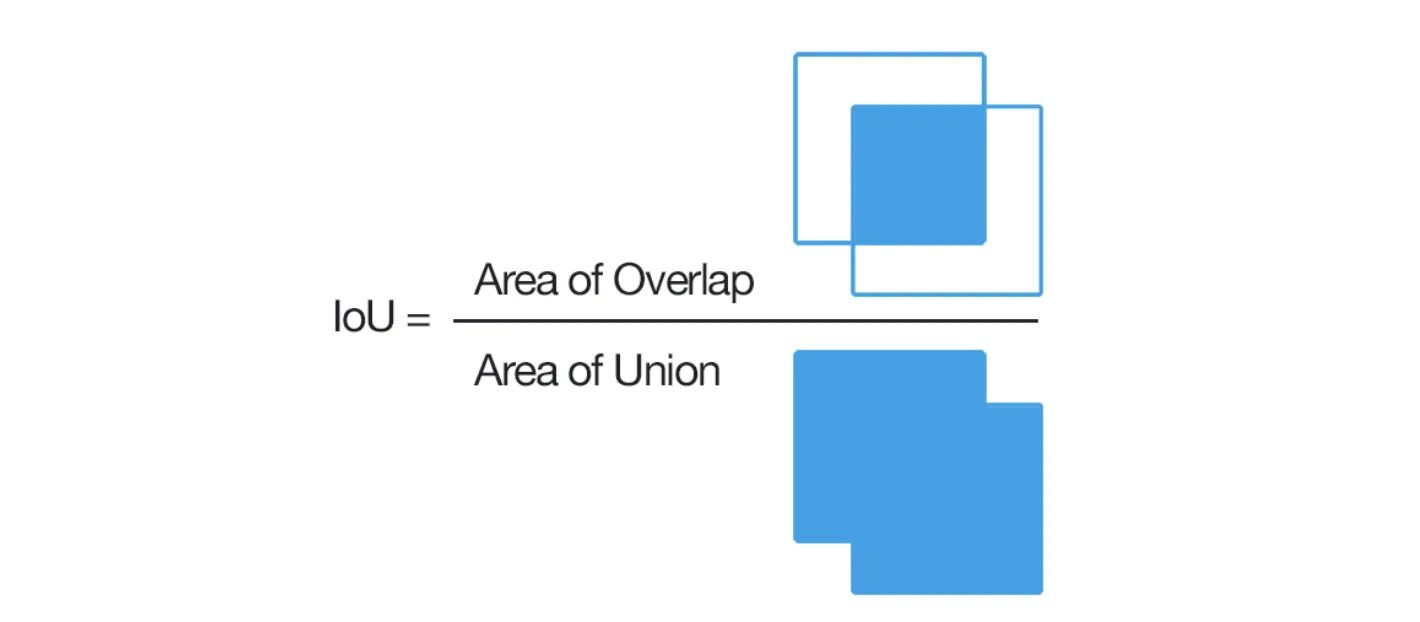
\includegraphics[width=0.8\textwidth]{images/IoU.jpg}
  \cite{IoU}
  \caption{Intersection over Union}
  \label{fig:IoU}
\end{figure}

\noindent
Per capire meglio, ecco alcuni esempi :
\begin{itemize}
    \item Se impostassimo la soglia IoU a 0,9, e la precision fosse pari al 16\% vorrà dire che solo 1 previsione su 6 corrisponde al punteggio;

    \item Con una soglia pari a 0,7, ed una precision del 65\% avrò che 4 previsioni sono al di sopra di tale punteggio.

    \item E se la soglia fosse del 0,3, e la precision salisse al 100\% vuol dire che tutte le previsioni hanno un IoU superiore a 0,3.
\end{itemize}

\noindent
Pertanto, la soglia IoU può influenzare significativamente il valore medio finale della Precisione Media. Questa dipendenza introduce variabilità nella valutazione del modello. Questo è negativo, perché può verificarsi uno scenario in cui un modello ottiene buoni risultati con una determinata soglia IoU e prestazioni nettamente inferiori rispetto ad un'altra.

Per contrastare questa debolezza, si è deciso di misurare la Precisione Media per ogni classe e per ogni soglia IoU, per poi calcolare la media dei punteggi ottenuti. \cite{mAP}

\section{Script}
Di seguito sono definite le operazioni necessarie, e specifiche per l'addestramento del modello base per la object detection YOLO26n.

\subsection{Dataset}
Il dataset utilizzato per il training di questo specifico modello YOLO è composto da una serie di immagini contenenti vari capi d'abbigliamento. Nello specifico, le annotazioni di questo dataset sono state generate tramite un ulteriore modello di segmentazione, chiamato SAM3, che verrà approfondito in seguito. \\
\noindent
Per la fase di inferenza è stato invece impiegato un dataset più ridotto. Poiché quest'ultimo comprendeva inizialmente alcune immagini già presenti nel set di training, è stata effettuata un'operazione di pulizia dei dati: tali immagini sono state rimosse dal dataset di addestramento, garantendo così una maggiore affidabilità nella valutazione qualitativa del modello.

\subsection{Training}

\subsubsection{Inizializzazione}

\begin{lstlisting}
import ultralytics
from ultralytics import YOLO
\end{lstlisting}

\subsubsection{Elaborazione}

\begin{lstlisting}
model = YOLO("yolo26n.pt")

trainArgs = {
    'data' : "dataset/dataset.yaml",
    'epochs' : 100,
    'imgsz' : 640,
    'batch' : 64,
    'device' : 0,
    'name' : "detection",
    'workers' : 4,
    'patience' : 10,
    'plots' : True,
}

model.train(**trainArgs)
\end{lstlisting}

\subsubsection{Parametri}
Dei parametri utilizzati nell'addestramento, i più rilevanti per le prestazioni sono :
\begin{itemize}
    \item epochs : numero di epoche
    \item batch size : numero di immagini alla volta che gli passo
    \item device : hardware che voglio utilizzare
    \item workers : numero di "lavoratori" CPU che mi aiutano in questo processo
\end{itemize}

\subsection{Risultati}
Alla fine della fase di addestramento, verranno prodotte delle statistiche che ci serviranno per la valutazione del nostro modello, cioè la precision, recall, F1 score e l'mAP.

\begin{figure}[htbp]
  \centering
  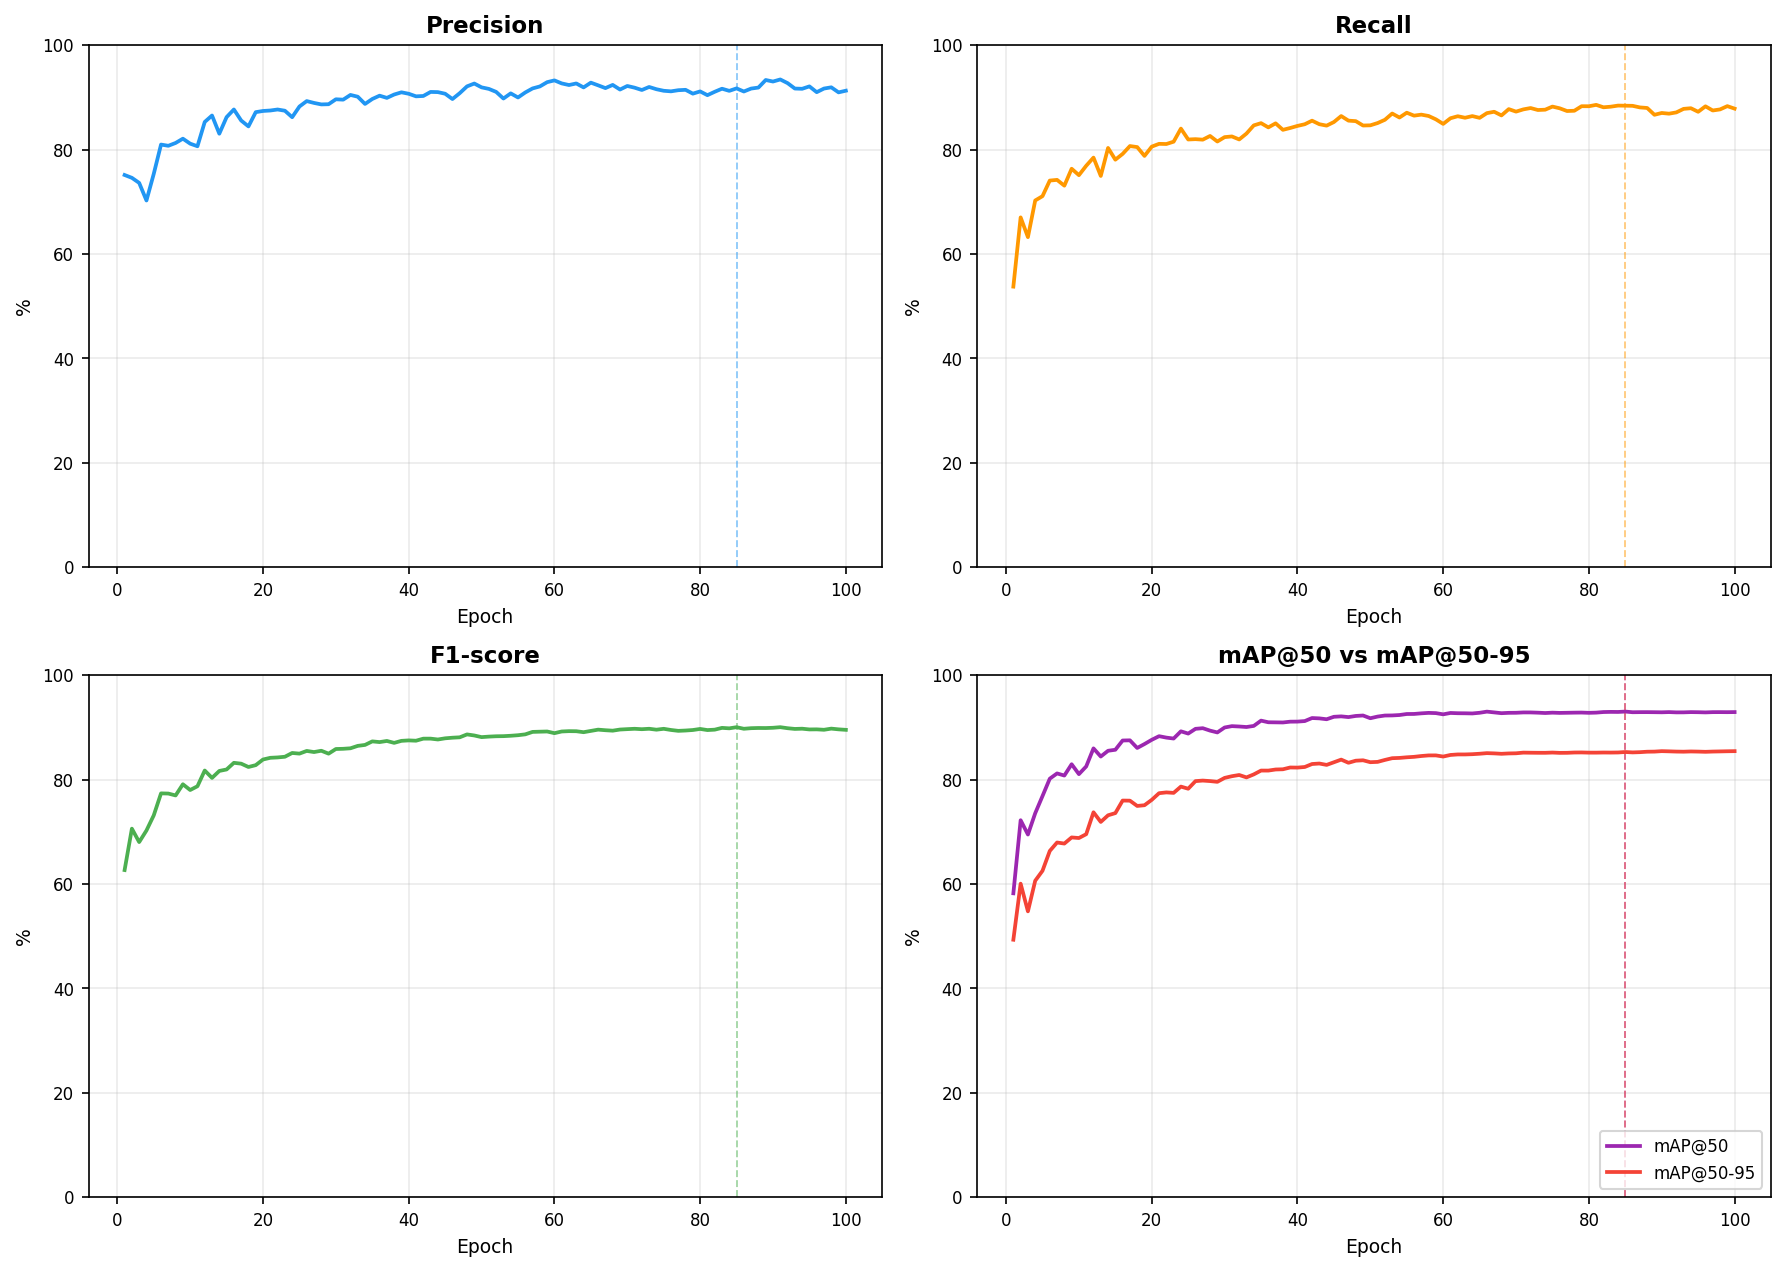
\includegraphics[width=0.8\textwidth]{images/training YOLO26n/training-stats.png}
  \caption{statistiche}
  \label{fig:statistiche}
\end{figure}

\noindent
Possiamo notare come inizialmente i grafici siano più rumorosi, e come invece più si va avanti nel numero di epoche, più la curva si stabilizzerà raggiungendo il suo plateau.

\newpage

\subsubsection{Confidence}
È il livello minimo di confidenza entro il quale il modello considera l'oggetto come valido. Questo è ottenuto andando a guardare il risultato dell'IoU e controllando che sia al sopra di questa soglia minima, che solitamente è impostata di default al 50\%. \\

\begin{figure}[h!]
  \centering
  \begin{minipage}[b]{0.49\textwidth}
    \centering
    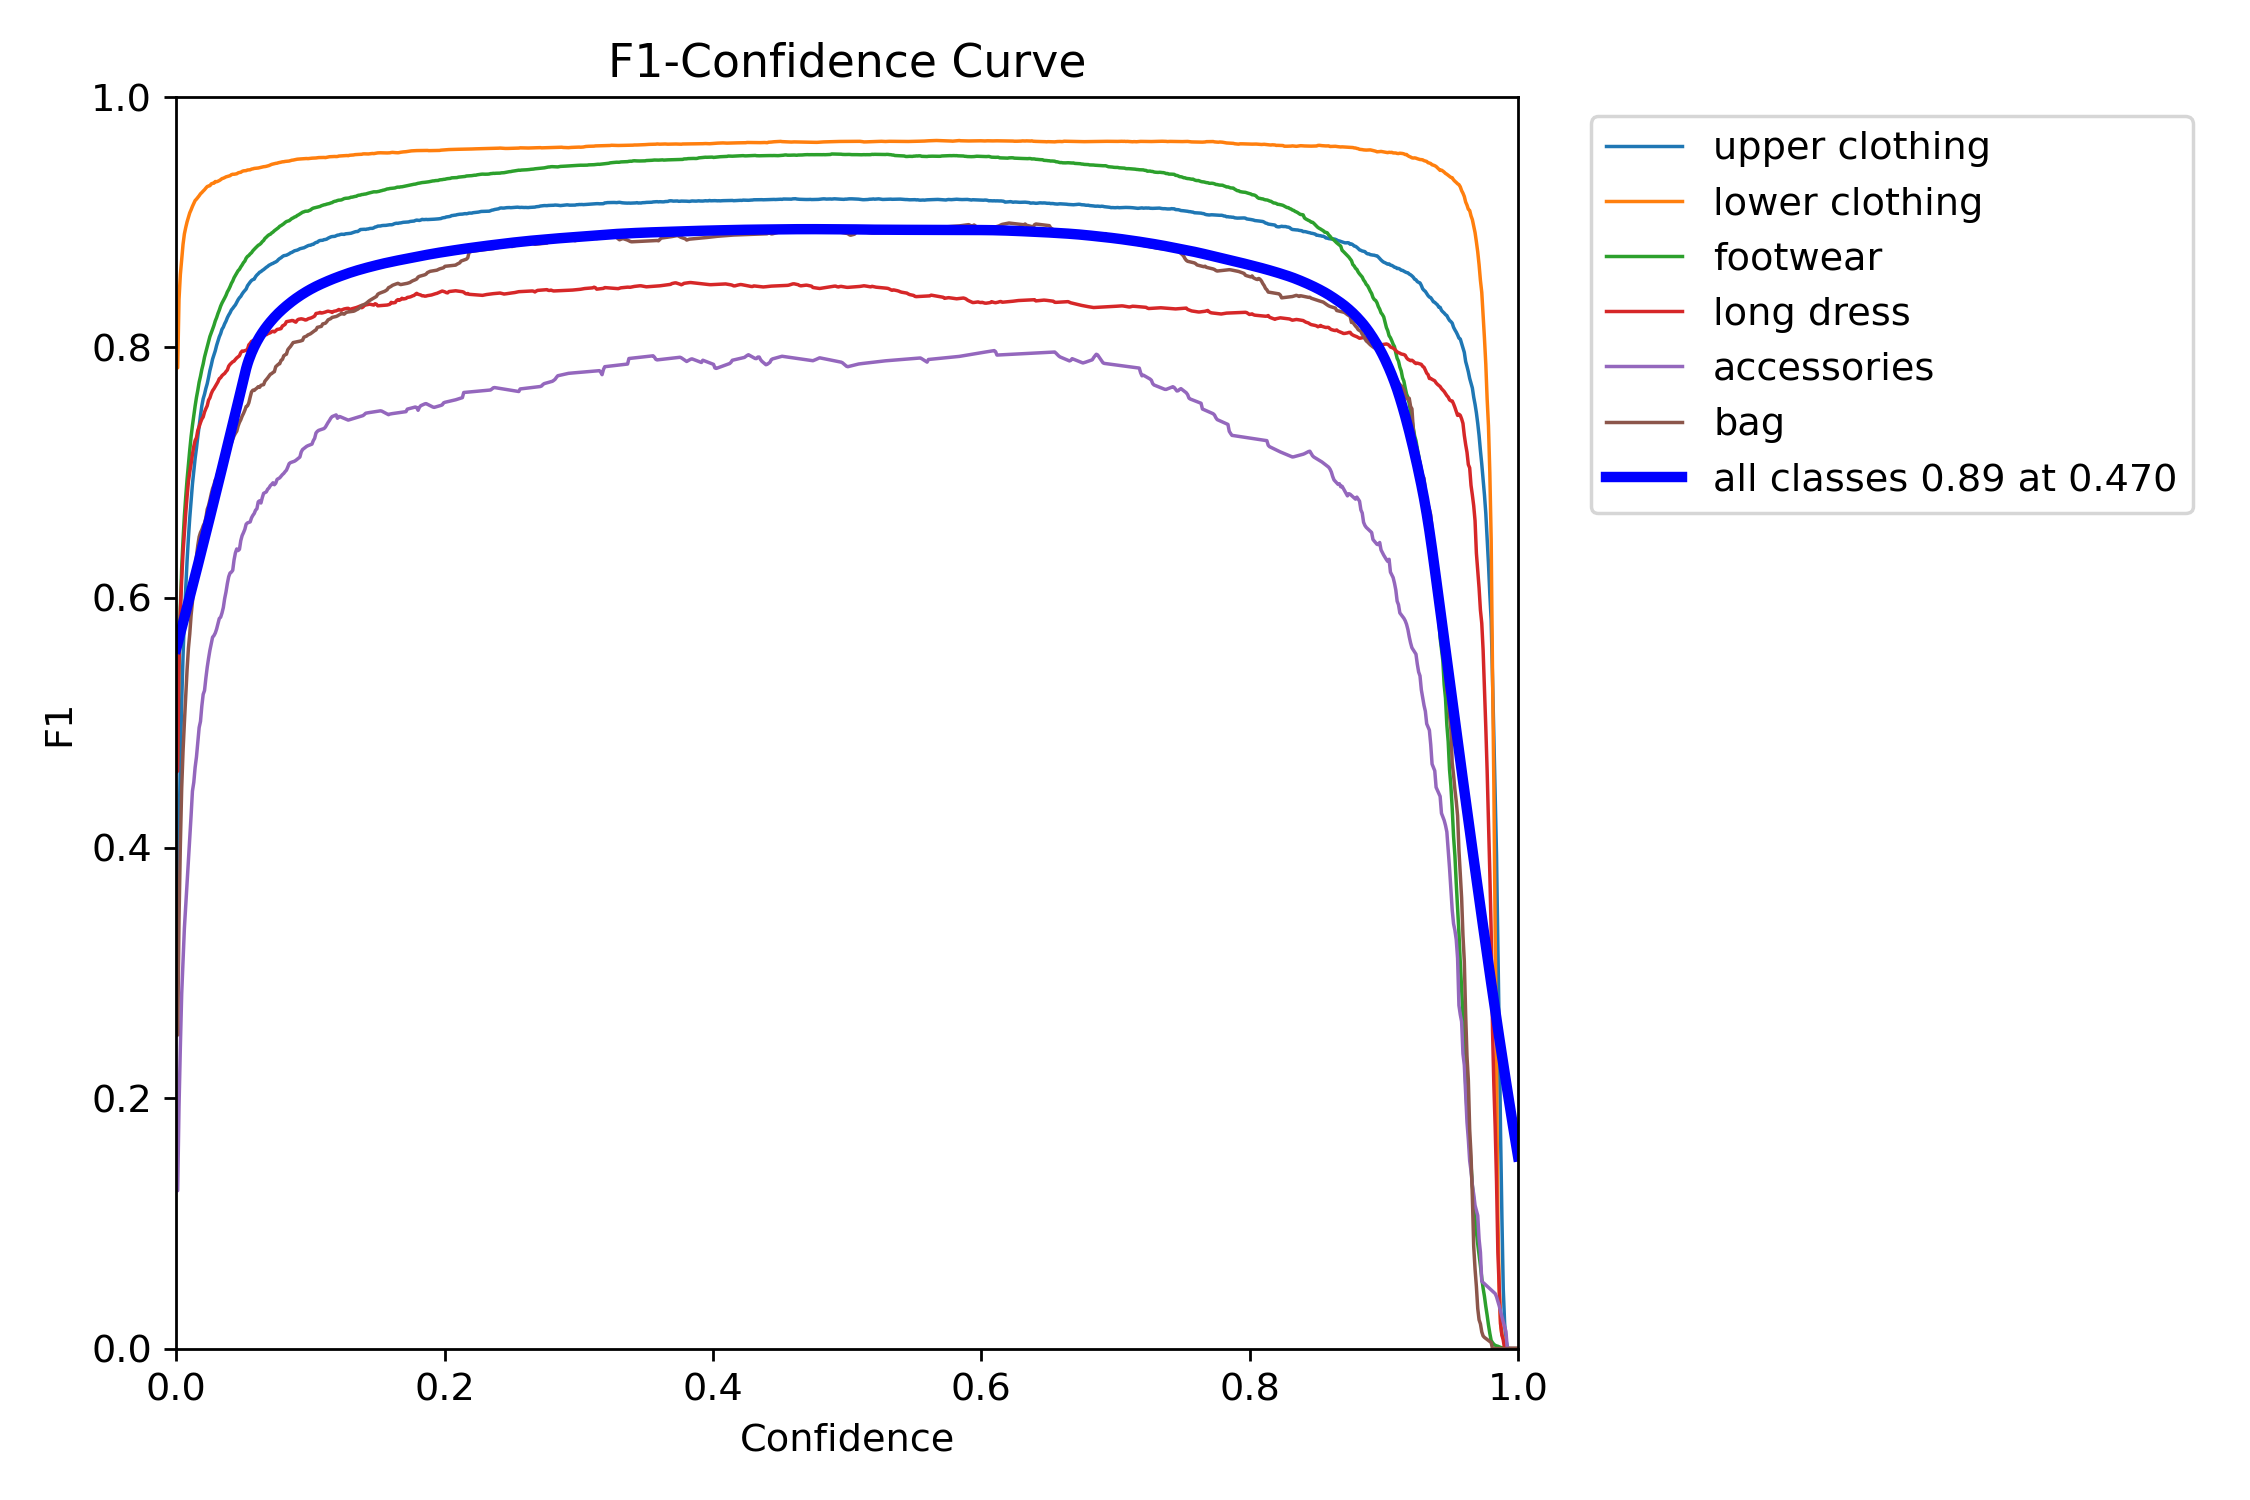
\includegraphics[width=\textwidth]{images/training YOLO26n/BoxF1_curve.png}
    \label{fig:f1_curve}
  \end{minipage}
  \hfill
  \begin{minipage}[b]{0.49\textwidth}
    \centering
    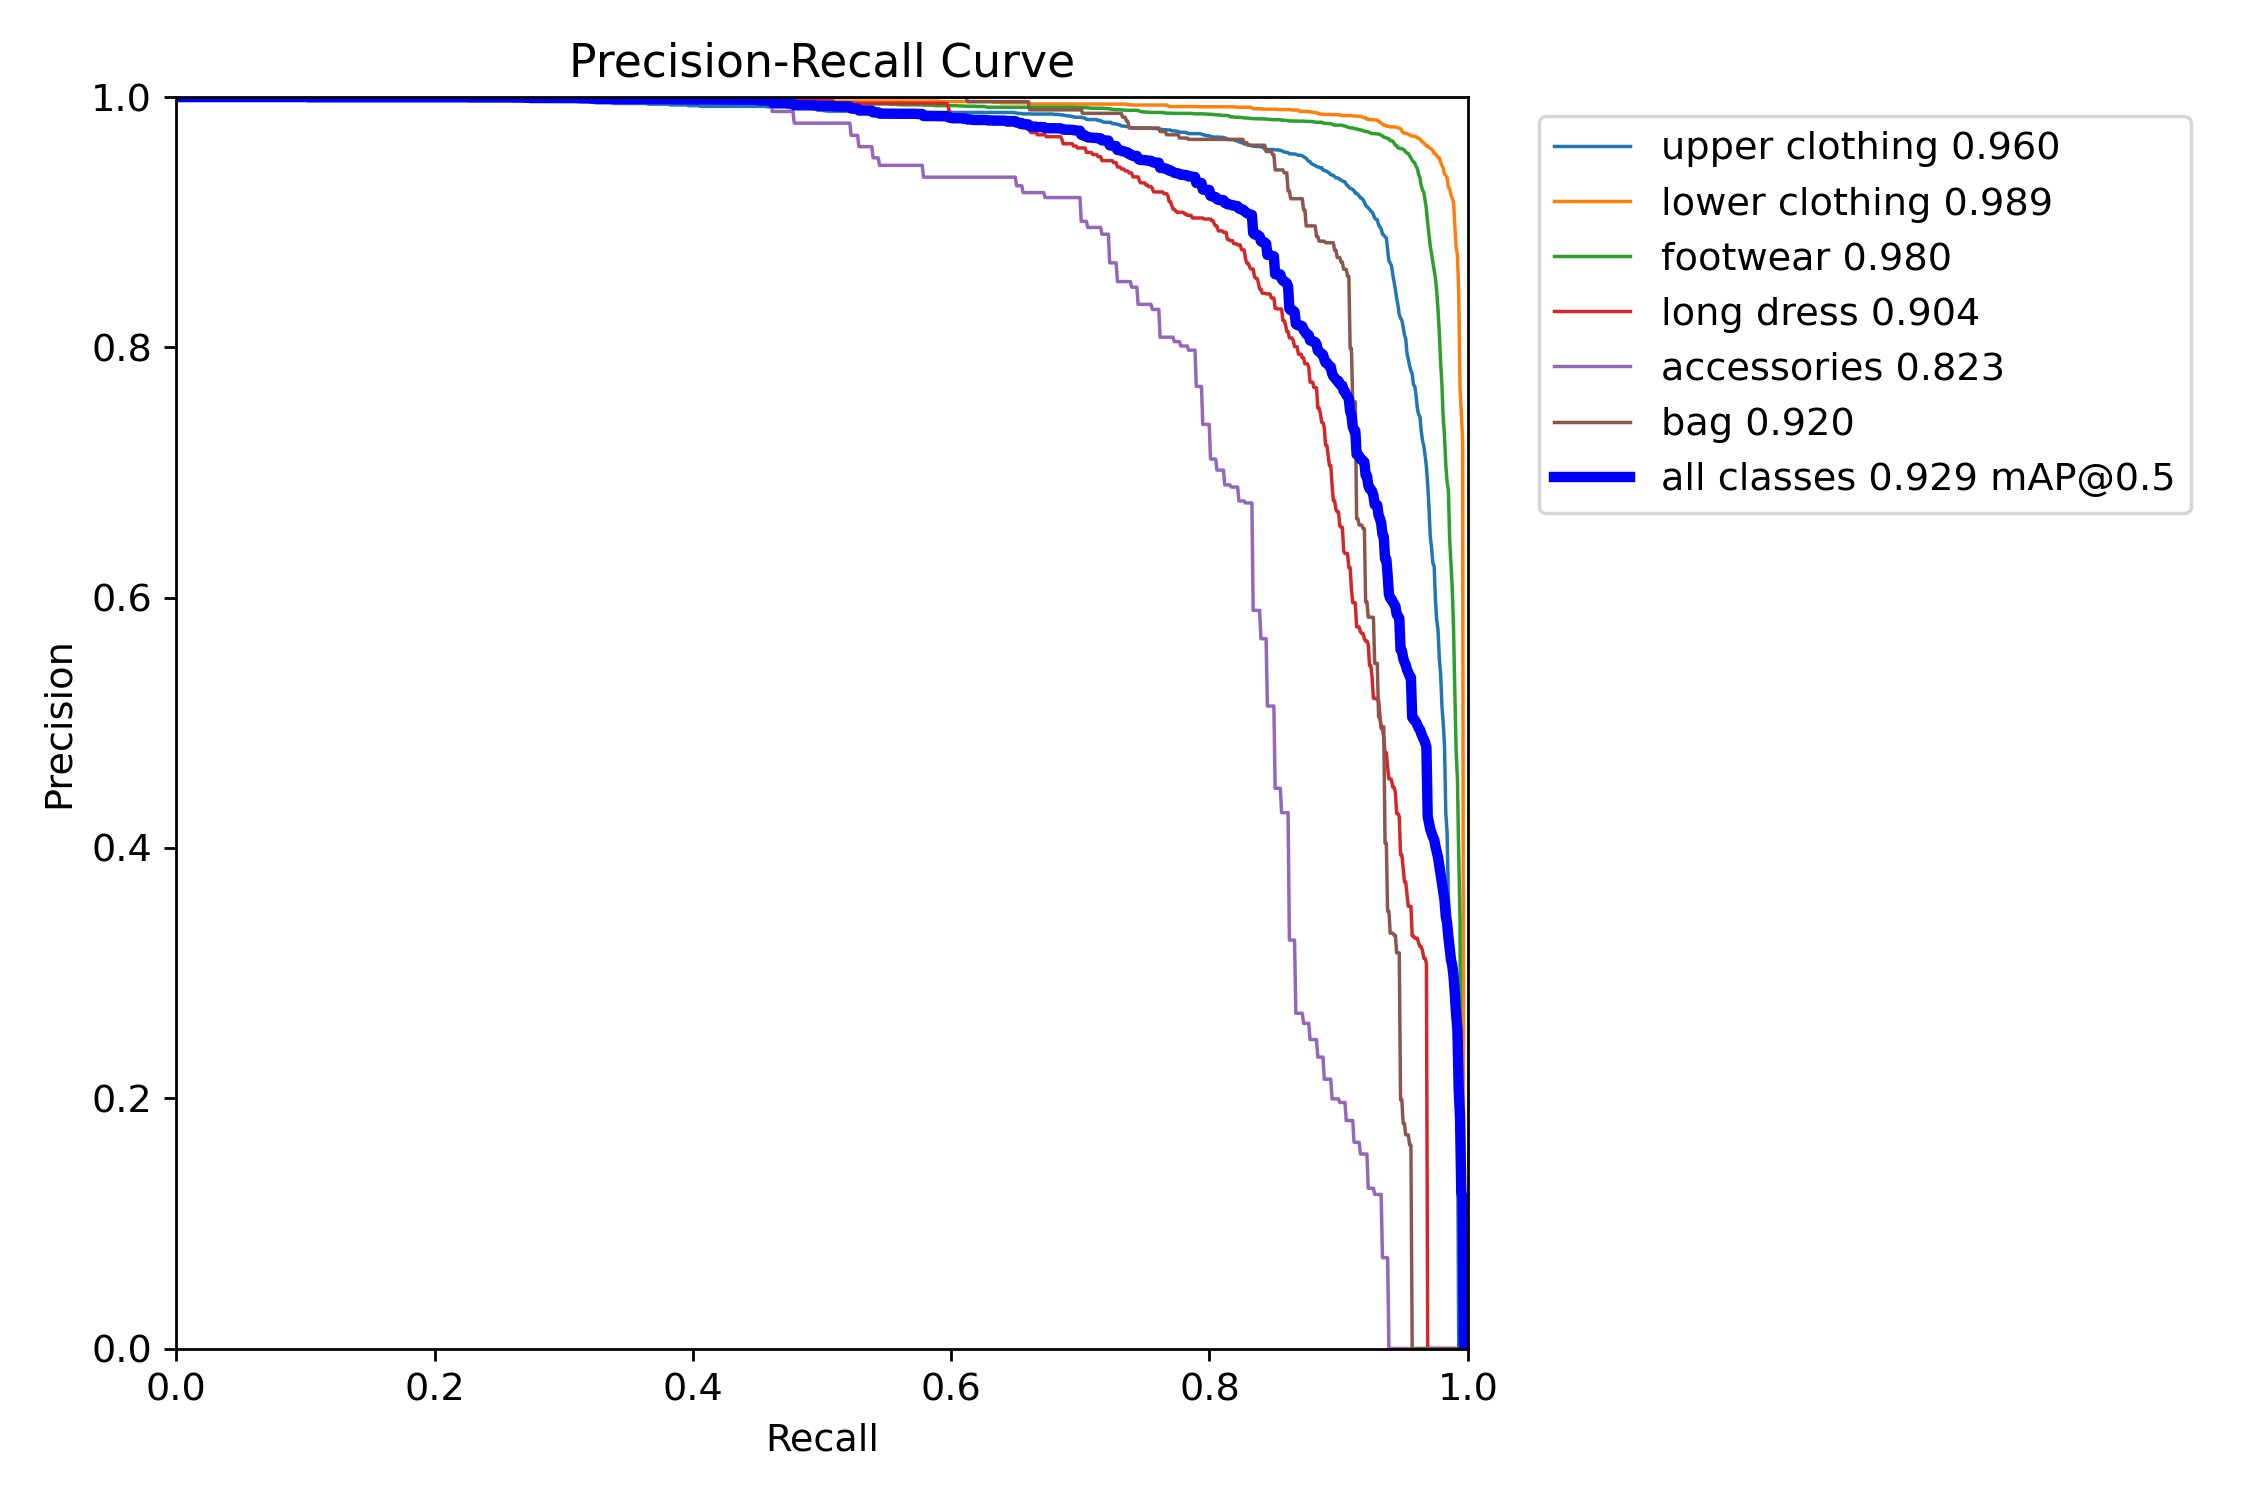
\includegraphics[width=\textwidth]{images/training YOLO26n/BoxPR_curve.png}
    \label{fig:pr_curve}
  \end{minipage}
\end{figure}

\noindent
Nel grafico a sinistra possiamo vedere che il punto massimo della curva F1, la quale rappresenta il punto ottimale in cui la soglia di confidence  fornisce il miglior compromesso tra precision e recall, è di 0.89 ottenuto  con confidence 0.470. \\
\noindent
Quindi il miglior bilanciamento tra la precision e la recall si otterrà impostando una confidence, cioè un limite di soglia, pari al 47\%.
Questo grafico è molto importante per scegliere il valore di confidence da fornire in fase di inferenza, dove appunto si minimizzano il più possibile i fenomeni di falso positivo (precision) e falso negativo (recall). \\

\noindent
In quello a destra, invece mostra la relazione fra precision e recall, con un valore di mAP50 pari a 0.929, e indica la media della precision agli intervalli di recall per tutte le classi, alla soglia di IoU di 0.5. \\
\noindent
In sostanza evidenzia il bilanciamento tra la capacità del modello di identificare in maniera corretta oggetti (precision) e la capacità di trovarli tutti (recall) per i vari livelli di soglia di confidenza.

\newpage

\subsubsection{Confusion matrix}

La confusion matrix mostra come il modello classifica le classi su cui è stato addestrato. \\

\begin{figure}[h!]
  \centering
  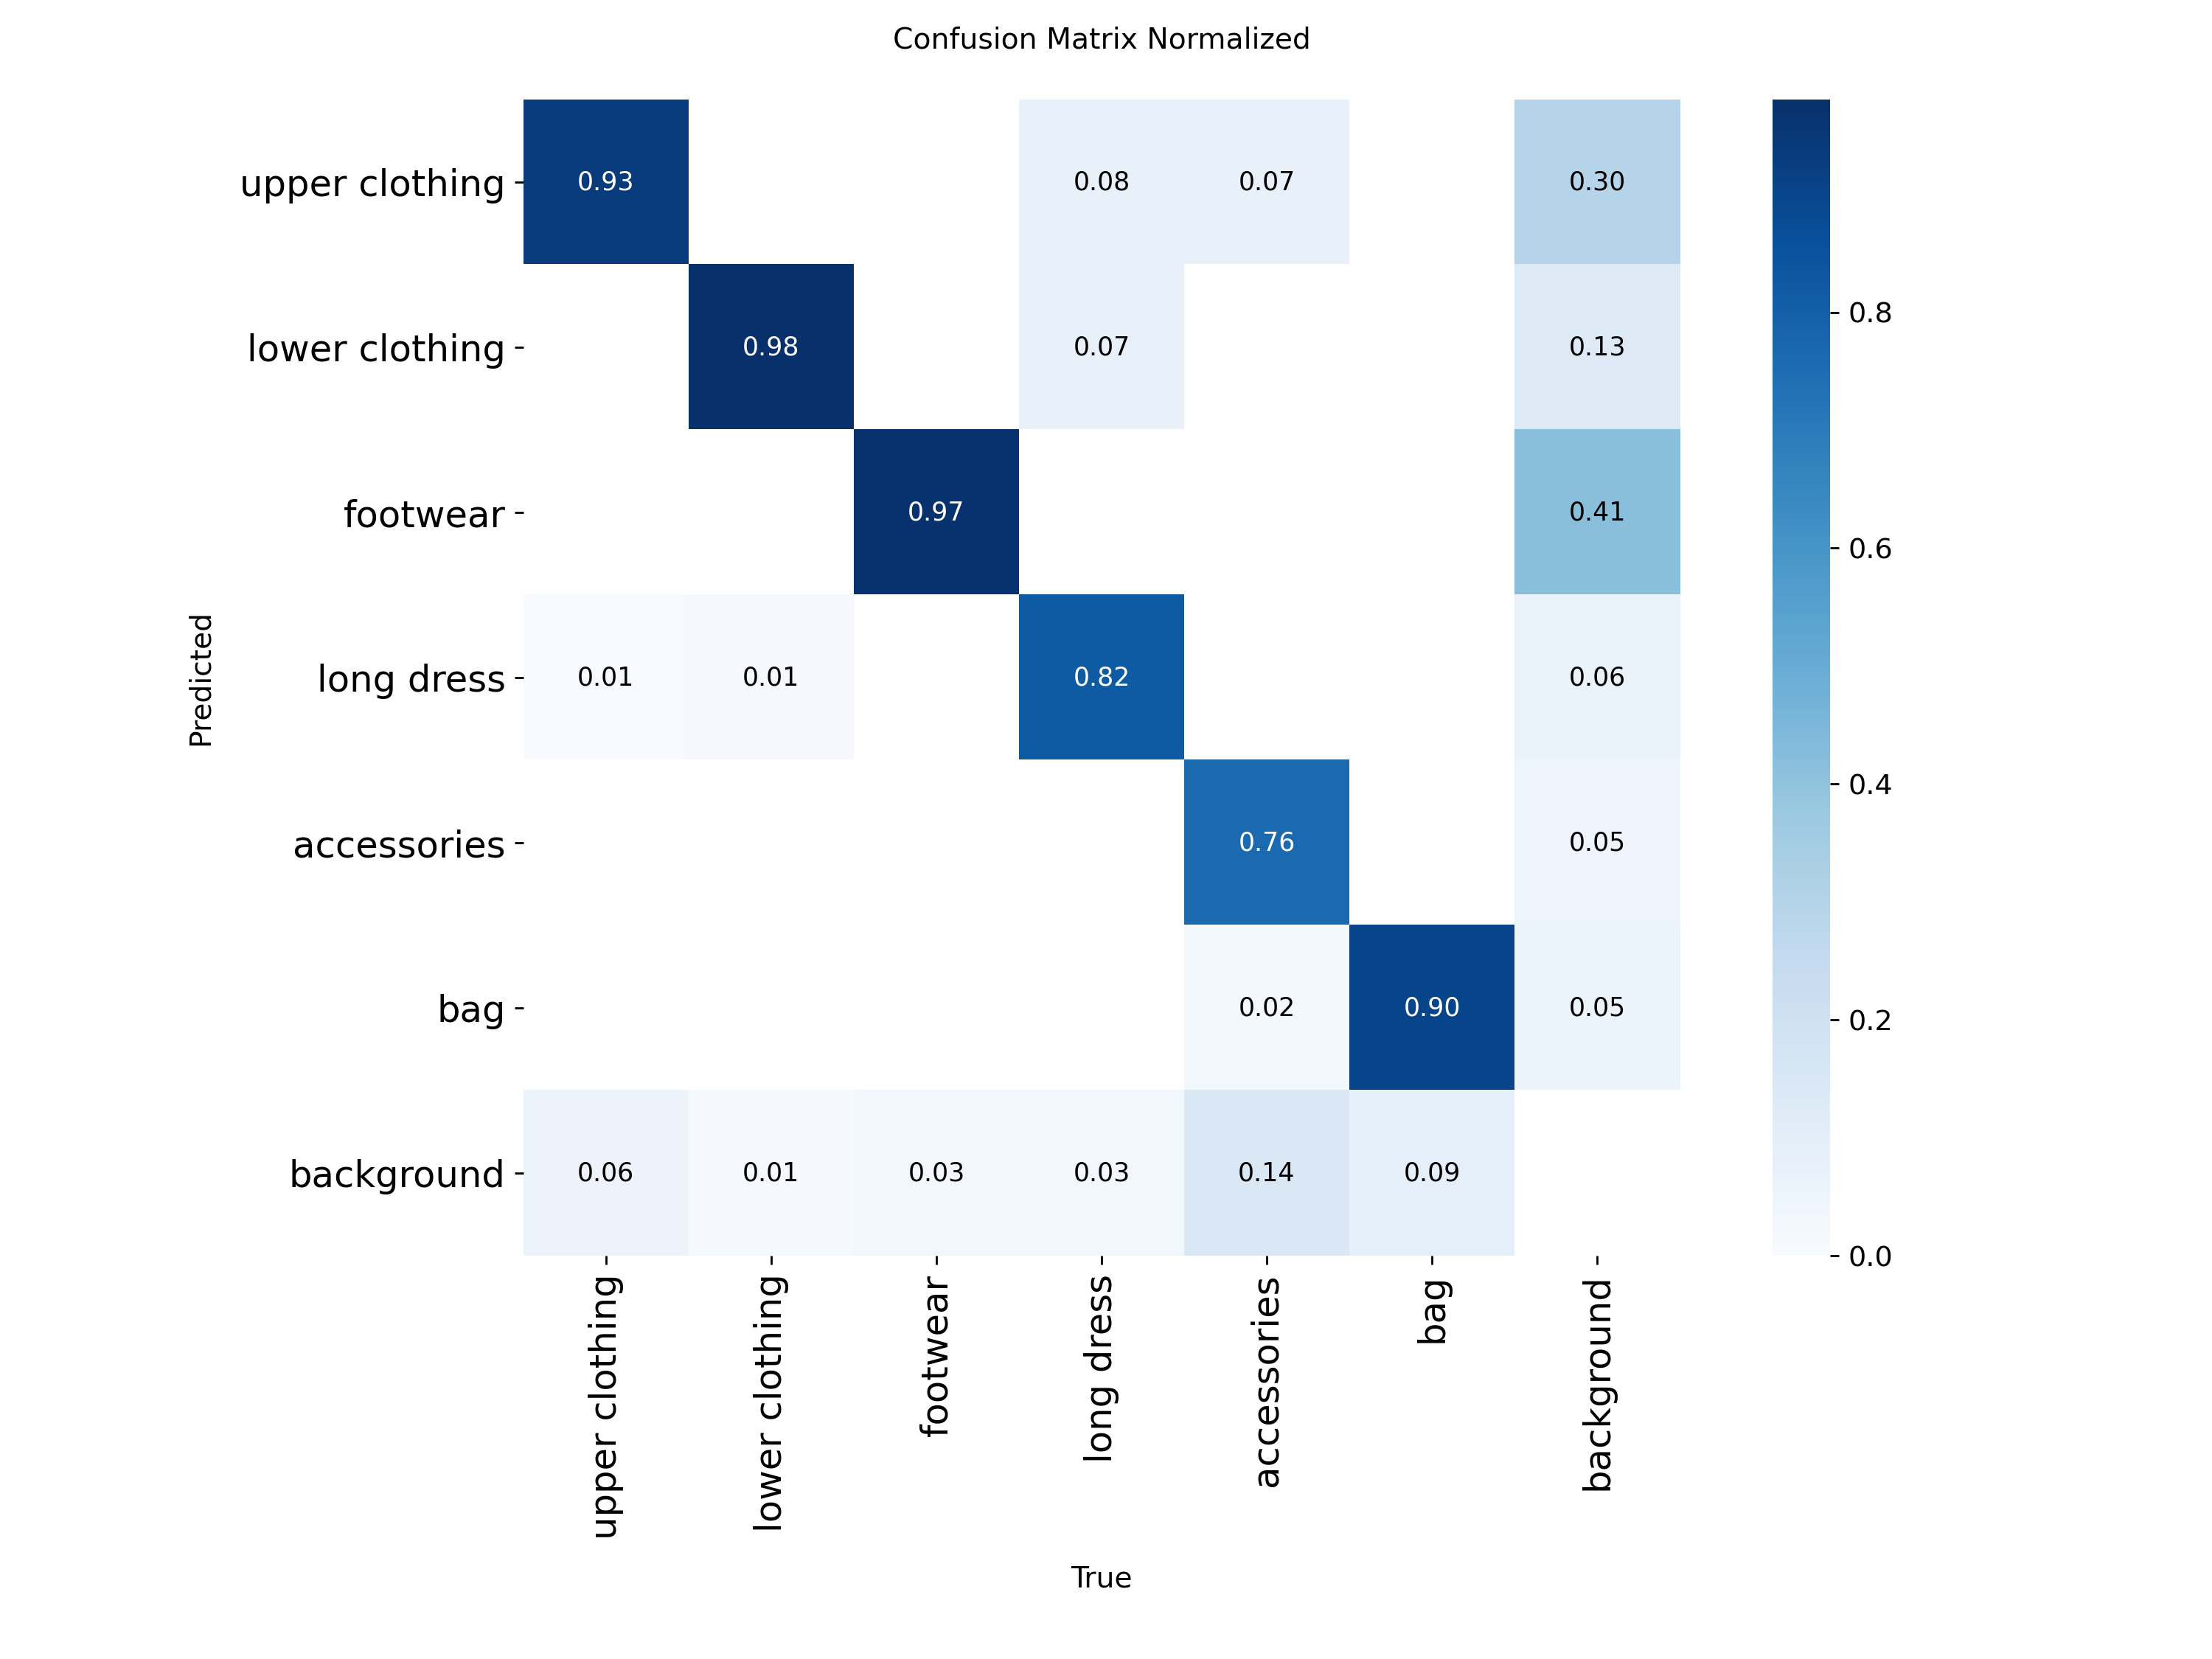
\includegraphics[width=0.8\textwidth]{images/training YOLO26n/confusion_matrix_normalized.png}
  \label{fig:confusion_matrix}
\end{figure}

\noindent
Il grafico può essere riassunto con alcune delle sue classi come :

\begin{itemize}
    \item Predicted "upper clothing" | True "upper clothing" : \\
        - il modello ha identificato correttamente il 93\% della categoria "upper clothing.
    \item Predicted "background" | True "accessories" : \\
        - il 14\% degli accessori è stato classificato come "background" (falso negativo).
    \item Predicted "footwear" | True "background" : \\
        - il 41\% del "background" è stato classificato come tale (vero negativo).
    \item Predicted "background" | True "background" : \\
        - nessun "background" è stato erroneamente classificato come capo d'abbigliamento (falso positivo assente).
\end{itemize}

\newpage

\subsection{Inferenza}

Dopo aver addestrato il modello con il nostro dataset, è possibile procedere con l'inferenza su altre immagini per verificare la presenza di alberi. Importante è soprattutto fare l'inferenza su un dataset diverso da quello utilizzato nella fase di training,, così da ottenere dei risultati più veritieri. \\
\noindent
È importante assicurarsi che le immagini in input siano dello stesso formato di quelle preparate per il training, in questo caso 640x640, devono quindi rispettare la risoluzione e la composizione dei channels RGB. \\

\noindent
Qui di seguito è dettagliata la funzione Python per l'inferenza con YOLO di Ultralytics, tramite la libreria OpenCV utilizzata in questo caso per lavorare con le immagini in input e output. \\

\begin{lstlisting}
def run(modelPath, imagesDir, outputDir="predictions", conf=0.25):
    model = YOLO(modelPath)
    Path(outputDir).mkdir(parents=True, exist_ok=True)

    for imgPath in Path(imagesDir).iterdir():
        img = cv2.imread(str(imgPath))
        if img is None:
            continue

        for result in model(img, conf=conf):
            for box in result.boxes.xyxy.cpu().numpy().astype(int):
                x1, y1, x2, y2 = box
                cv2.rectangle(img, (x1, y1), (x2, y2), (0, 255, 0), 2)

        cv2.imwrite(f"{outputDir}/{imgPath.stem}_result.jpg", img)
\end{lstlisting}

\vspace{0.5cm}
\noindent
Questa funzione implementa la fase di inferenza del modello YOLO26 su un insieme di immagini. Dato il percorso dei pesi addestrati e quello della cartella di input, il modello viene caricato tramite la libreria Ultralytics e applicato iterativamente a ciascuna immagine, con una soglia di confidenza configurabile che filtra le predizioni meno affidabili. \\
\noindent
Per ogni immagine vengono estratte le bounding box predette, sovrapposte all'immagine originale e il risultato viene salvato in una cartella di output dedicata, consentendo così una verifica qualitativa delle detection prodotte dal modello.
